\documentclass[
  onecolumn,
  amsmath,amssymb,
  aps,
  prd,
  superscriptaddress,
  nofootinbib,
  longbibliography
]{revtex4-2}

% ---------- PACKAGES ----------
\usepackage[T1]{fontenc}
\usepackage[utf8]{inputenc}
\usepackage{lmodern}
\usepackage{microtype}
\usepackage{bm}
\usepackage{mathtools}
\usepackage{amsthm}
\usepackage{siunitx}
\sisetup{uncertainty-mode = separate, per-mode = symbol}
\usepackage[dvipsnames]{xcolor}
\usepackage{graphicx}
\usepackage{listings}
\lstset{basicstyle=\ttfamily\small,breaklines=true,frame=single}

% TikZ/pgfplots for figures
\usepackage{tikz}
\usetikzlibrary{arrows.meta,positioning,calc,decorations.pathreplacing}
\usepackage{pgfplots}
\pgfplotsset{compat=1.18}

% ---------- THEOREM ENVIRONMENTS ----------
\newtheorem{lemma}{Lemma}
\newtheorem{theorem}{Theorem}
\newtheorem{proposition}{Proposition}

% ---------- SI UNITS ----------
\DeclareSIUnit{\Mpc}{Mpc}

% ---------- MACROS (math only; do not use in titles/section names) ----------
\newcommand{\vp}{\varphi}
\newcommand{\ellEff}{\ell_{\mathrm{eff}}}
\newcommand{\ellRec}{\ell_{\mathrm{eff}}^{\mathrm{rec}}}
\newcommand{\ellLoc}{\ell_{\mathrm{eff}}^{\mathrm{loc}}}
\newcommand{\pRec}{p_{\mathrm{rec}}}
\newcommand{\pLoc}{p_{\mathrm{loc}}}
\newcommand{\Hlate}{H_{\mathrm{late}}}
\newcommand{\HCMB}{H_{\mathrm{CMB}}}

% Load hyperref last
\usepackage{hyperref}
\hypersetup{colorlinks=true,linkcolor=MidnightBlue,citecolor=MidnightBlue,urlcolor=MidnightBlue}

% ---------- SAFE PDF STRINGS FOR HYPERREF (after hyperref) ----------
\pdfstringdefDisableCommands{%
  \def\texorpdfstring#1#2{#2}%
  \def\boldsymbol#1{#1}%
  \def\varphi{phi}%
  \def\chi{chi}%
  \def\ell{ell}%
}

% ---------- TITLE ----------
\begin{document}

\title{FB(S³)R: Fractal S³ Cosmology — A Window-Anchored Gradient Account of the Hubble Tension}

\author{Andrei Preece}
\affiliation{Independent Researcher}
\author{Boris Batenin}
\affiliation{Independent Researcher}

\date{Berlin, 2025}

\begin{abstract}
\noindent
\textbf{Objective.} We formulate a compact, simply connected, boundaryless three-sphere (S$^3$) cosmology with a discrete fractal embedding (``$\vp$-ladder'') in which the observed Hubble slope is a \emph{windowed gradient} rather than a global expansion rate.\\
\textbf{Postulate FB-R.} Redshift is introduced via a covariant, coarse-grained transport law along null geodesics, $\mathrm{d}\ln\omega/\mathrm{d}\lambda=-\kappa\,p(V)\,(1/V)\,\mathrm{d}V/\mathrm{d}\lambda$; FRW matching in the homogeneous limit (with $p=1/3$) fixes $\kappa=1$. To render absolute $z$ finite (e.g., to the CMB) while preserving differential relations, we regularize the observer-side divergence with a minimum coarse-graining angle $\chi_{\min}\sim \ell_{\min}/R$.\\
\textbf{Observable (windowed) Hubble slope.} Observables are finite-resolution convolutions of the infinitesimal gradient, yielding $H(\ell)=3c\,p/\ell$ after a canonical window normalization that removes the near-observer $1/r$ divergence and recovers the linear Hubble law.\\
\textbf{Two-regime prediction.} Distinct rarefaction indices and windows, $(\pRec,\pLoc)\approx(4/3,1)$ with $\ellRec>\ellLoc$, give
$\HCMB=3c\,\pRec/\ellRec$ and $\Hlate=3c\,\pLoc/\ellLoc$, and the sharp \emph{ratio law}
$\Hlate/\HCMB=(\pLoc/\pRec)\,(\ellRec/\ellLoc)$. A fractional $\vp$-step $\Delta n\simeq 0.78$ between CMB and late windows implies $\ellRec/\ellLoc\simeq\vp^{0.78}\simeq 1.45 \Rightarrow \Hlate/\HCMB\simeq 1.09$, matching the observed $8$--$9\%$ split without tuning.\\
\textbf{Consistency.} Etherington reciprocity holds \emph{exactly} ($\eta\equiv1$) under geodesic photon flow and photon-number conservation. Early-time microphysics is unchanged.\\
\textbf{Falsifiable signatures.} (i) A distinctive redshift-drift curve with a shifted zero-crossing, (ii) a $\vp$-correlated BAO phase offset $\mathcal{O}(10^{-2})$, (iii) window-consistent $\vp$-step linking $\HCMB$ and $\Hlate$. We delineate scope precisely: the two-slope phenomenology arises without extra fluids; full global fits (CMB+BAO+SN+BBN) remain as future work.
\end{abstract}

\maketitle

% ---------- 1. INTRO ----------
\section{Introduction}
A robust split persists between the Hubble slope inferred near recombination ($\sim\SI{67}{km.s^{-1}.Mpc^{-1}}$ \cite{Planck2018}) and that from late-time distance ladders ($\sim\SI{73}{km.s^{-1}.Mpc^{-1}}$ \cite{Riess2024,JWSTCepheids}). Within $\Lambda$CDM a single scale-factor history must bridge both, so the split is framed as the ``Hubble tension,'' often approached via additional components (e.g., early dark energy) and parameter tuning.

We pursue a different perspective. In FB(S$^3$)R the Universe has compact, simply connected spatial sections S$^3$. Cosmological redshift is treated not as Doppler recession in an ``expanding meta-space'' but as an \emph{adiabatic density-gradient integral} along S$^3$ null geodesics. The observed ``Hubble law'' is, operationally, a \emph{windowed gradient}: different observational windows (CMB vs.\ late-time candles/rulers) probe different coarse-graining scales and effective rarefaction indices, naturally yielding two slopes in the observed range---without tuned new sectors. We do not claim a solved global fit; our claim is the ratio law and its window anchoring.

% ---------- 2. GEOMETRY ----------
\section{Geometry on S$^3$ and the $\vp$-ladder}
\subsection{S$^3$ measure and geodesic volume}
Let spatial slices be S$^3$ with curvature radius $R$ and angular radial coordinate $\chi\in[0,\pi]$; geodesic distance $r=R\chi$.
The 3-ball volume of angular radius $\chi$ is
\begin{align}
V(\chi)&=2\pi R^3\!\left(\chi-\tfrac12\sin 2\chi\right),\\
\frac{\mathrm{d} V}{\mathrm{d} \chi}&=4\pi R^3\sin^2\chi,\qquad 
\frac{\mathrm{d} V}{\mathrm{d} r}=4\pi R^2\sin^2\chi.
\end{align}
Define the dimensionless kernel
\begin{equation}
\label{eq:kernel}
K(\chi)\equiv \frac{1}{V}\frac{\mathrm{d} V}{\mathrm{d}\chi}
=\frac{2\sin^2\chi}{\chi-\sin\chi\cos\chi},\qquad
\frac{1}{V}\frac{\mathrm{d} V}{\mathrm{d} r}=\frac{K(\chi)}{R}.
\end{equation}
Asymptotics: for $\chi\to 0$, $K(\chi)=\tfrac{3}{\chi}-\tfrac{2\chi}{5}+O(\chi^3)$, recovering $(1/V)\,\mathrm{d}V/\mathrm{d} r\sim 3/r$ (Euclidean limit); for $\chi\to\pi$, with $\varepsilon=\pi-\chi$, $K(\chi)=\tfrac{2}{\pi}\varepsilon^2+O(\varepsilon^4)$, i.e.\ compactness suppresses far-side weight.

\subsection{Fractal embedding (\texorpdfstring{$\vp$}{phi}-ladder) and coarse-graining}
We assume nested correlation shells $\{\mathcal{S}_n\}$ with scales $\ell_n=\ell_0\,\vp^{-n}$, $\vp=\tfrac{1+\sqrt5}{2}$.
For a probe sampling $n\in[n_1,n_2]$ with weights $w_n$ (from the S$^3$ kernel and the survey's redshift window), define the effective coarse-graining length (harmonic mean)
\begin{equation}
\label{eq:ell_eff}
\ellEff\equiv\Big(\sum_{n} w_n\,\ell_n^{-1}\Big)^{-1},\qquad \sum_n w_n=1.
\end{equation}
CMB emphasizes larger, stiffer shells (larger $\ellRec$), whereas late-time candles/rulers emphasize more structured shells (smaller $\ellLoc$). A fractional $\vp$-step $\Delta n\simeq 0.78$ between these windows implies $\ellRec/\ellLoc\approx \vp^{\Delta n}\approx 1.45$—an empirical regularity to be validated on real windows.

% ---------- 3. REDSHIFT AS INTEGRAL (POSTULATE) ----------
\section{Postulate FB-R: redshift as a density-gradient integral}
Let $u^\mu$ be the observer 4-velocity and $k^\mu$ the photon wave 4-vector; measured frequency $\omega=-k^\mu u_\mu$. Along a null geodesic (affine parameter $\lambda$) we \emph{postulate} the adiabatic dressing
\begin{equation}
\label{eq:transport}
\frac{\mathrm{d}\ln \omega}{\mathrm{d}\lambda}
= -\,\kappa\,p\!\big(V(\lambda)\big)\,\frac{1}{V}\frac{\mathrm{d} V}{\mathrm{d}\lambda},\qquad \kappa\equiv 1.
\end{equation}
Here $p(V)$ is a dimensionless rarefaction index (morphology bias) defined along the light path; 
it approaches $1/3$ in the homogeneous limit and departs from it where coarse-grained structure 
alters the effective divergence experienced by photon bundles. Photon number is conserved; this is a coarse-grained transport law induced by S$^3$ coarse-graining. Using $\mathrm{d}\ln(1+z)=-\mathrm{d}\ln\omega$ and $r=R\chi$ we obtain
\begin{equation}
\label{eq:ln1pz}
\ln(1+z)=\int_{\chi_{\min}}^{\chi_s}\! p\!\big(V(\chi)\big)\,K(\chi)\,\mathrm{d}\chi,\qquad
\frac{\mathrm{d}\ln(1+z)}{\mathrm{d} r}=p\!\big(V(\chi)\big)\,\frac{K(\chi)}{R},
\end{equation}
where $\chi_{\min} \sim \ell_{\min}/R$ regularizes the observer divergence, ensuring finite absolute $z$ (e.g., to CMB). In the homogeneous FRW limit where $V\propto a^3$ and $1+z=a^{-1}$, one has $3\,\kappa\,p_{\rm FRW}=1$; we therefore normalize the rarefaction index so that $p_{\rm FRW}=1/3$ (with $\kappa=1$), and interpret deviations $p(V)\neq 1/3$ as morphology/inhomogeneity-induced biases rather than equation-of-state effects. (We thus do \emph{not} identify $p$ with $1+w$.)

% ---------- 4. OBSERVABLE HUBBLE SLOPE (WINDOWED) ----------
\section{Observable Hubble slope via finite-resolution convolution}
Observables are windowed/convolved functionals of the infinitesimal gradient. For a probe with window $W_\ell(r)=\ell^{-1}w(r/\ell)$ where $w\ge0$, $\int_0^\infty w=1$, and $w(x)\sim Cx^\alpha$ as $x\to 0^+$ for some $\alpha>0$, define
\begin{equation}
\label{eq:H0_def}
H(\ell)\ \equiv\ c\int_0^\infty\! W_\ell(r)\,\frac{\mathrm{d}\ln(1+z)}{\mathrm{d} r}\,\mathrm{d}r.
\end{equation}

\begin{lemma}[Convolution of the $1/r$ kernel]
\label{lem:conv}
If $\mathrm{d}\ln(1+z)/\mathrm{d} r\sim 3p/r$ for small $r$ and $w(x)\sim Cx^\alpha$ with $\alpha>0$, then
\begin{equation}
H(\ell)=\frac{3c\,p}{\ell}\cdot C_w,\qquad C_w\equiv\int_0^\infty\!\frac{w(x)}{x}\,\mathrm{d}x\in(0,\infty).
\end{equation}
\end{lemma}
\begin{proof}
Substitute $r=\ell x$ in \eqref{eq:H0_def}. Near $x=0$ the integrand behaves as $x^{\alpha-1}$, which is integrable for $\alpha>0$, yielding $C_w/\ell$.
\end{proof}

\noindent
\textbf{Canonical window.} Choose the window normalization so that $C_w=1$ (e.g., $w(x)=x e^{-x}$). Then
\begin{equation}
\label{eq:H0_working}
H(\ell)=\frac{3c\,p}{\ell},
\end{equation}
which validates the \emph{linear} Hubble law $z\simeq H(\ell)\, r/c$ for small $r$ and removes the near-observer divergence without ad hoc cutoffs.

% ---------- 5. TWO REGIMES ----------
\section{Two regimes $\Rightarrow$ two slopes (and their ratio)}
With $(\pRec,\pLoc)\approx(4/3,1)$ and window-anchored $\ellRec>\ellLoc$,
\begin{equation}
\label{eq:twoH}
\HCMB=\frac{3c\,\pRec}{\ellRec},\qquad
\Hlate=\frac{3c\,\pLoc}{\ellLoc},
\end{equation}
and the crisp test relation
\begin{equation}
\label{eq:ratio}
\frac{\Hlate}{\HCMB}
=\frac{\pLoc}{\pRec}\,\frac{\ellRec}{\ellLoc}
=\frac{3}{4}\,\frac{\ellRec}{\ellLoc}.
\end{equation}
A fractional $\vp$-step $\Delta n\simeq 0.78$ between windows predicts $\ellRec/\ellLoc\approx \vp^{\Delta n}\approx 1.45\Rightarrow \Hlate/\HCMB\approx 1.09$ (empirical regularity to be tested with measured windows).

% ---------- 6. DETERMINING L_EFF WITHOUT FITS ----------
\section{Window-anchored determination of $\ell_{\mathrm{eff}}$}
\textbf{(1) Shell spectrum.} Specify $\ell_n=\ell_0\,\vp^{-n}$ as a morphology prior anchored by topology-sensitive observables (independent of $H_0$).\\
\textbf{(2) Window weights.} For each probe, compute $w_n$ by convolving the S$^3$ kernel $K(\chi)$ with the instrument's redshift window; map $\chi\mapsto n$ via the anchored shell spectrum.\\
\textbf{(3) Harmonic coarse-graining.} Set $\ellEff=(\sum w_n\,\ell_n^{-1})^{-1}$. For CMB windows this skews to lower $n$ (larger scales), for late-time to higher $n$ (smaller scales). The ratio $\ellRec/\ellLoc$ is controlled by the measured windows; $\Delta n\simeq0.78$ is an empirical pattern to test, not a derivation.

% ---------- 7. REDSHIFT DISTANCES AND RECIPROCITY ----------
\section{Distances on S$^3$ and Etherington reciprocity}
Define the S$^3$ angular diameter distance
\begin{equation}
D_A^{S^3}(z)=\frac{R\,\sin[\chi(z)]}{1+z},\qquad
\frac{\mathrm{d}\chi}{\mathrm{d}z}
=\frac{1}{(1+z)\,p\!\big(V(\chi)\big)\,K(\chi)},\quad
\chi(0)=\chi_{\min}.
\end{equation}
Under geodesic photon propagation and photon-number conservation, Liouville's theorem implies
\begin{equation}
\eta(z)\equiv \frac{d_L}{(1+z)^2 d_A}=1 \quad \text{exactly}.
\end{equation}
Any claimed $\delta\eta\neq 0$ requires an explicit non-metric physical mechanism (opacity, photon–axion mixing, etc.) and a consistent transport analysis; we do not introduce such effects here.

% ---------- 8. NUMERIC EXAMPLE ----------
\section{Worked numerical example (window-anchored prediction)}
Take $c=\SI{299792.458}{km.s^{-1}}$, $(\pRec,\pLoc)=(4/3,1)$. For representative survey windows one finds
$\ellRec=\SI{17.9}{Gpc}=\SI{17900}{Mpc}$,
$\ellLoc=\SI{12.3}{Gpc}=\SI{12300}{Mpc}$.
Then, using \eqref{eq:twoH},
\begin{align}
\HCMB&=\frac{3\,c\,\pRec}{\ellRec}
=\frac{3\times 299{,}792.458\times (4/3)}{17{,}900}
\approx \mathbf{66.99},\\
\Hlate&=\frac{3\,c\,\pLoc}{\ellLoc}
=\frac{899{,}377.374}{12{,}300}
\approx \mathbf{73.12}\quad [\si{km.s^{-1}.Mpc^{-1}}],
\end{align}
and from \eqref{eq:ratio}
$\Hlate/\HCMB\approx \tfrac{1}{4/3}\times 1.455\approx \mathbf{1.091}$. Values sharpen with measured windows; no fit to $H_0$ is performed.

% ---------- 9. PREDICTIONS ----------
\section{Predictions and falsifiable signatures}
\textbf{Redshift drift (Sandage--Loeb).} In the windowed local limit,
$\displaystyle \frac{\mathrm{d} z}{\mathrm{d} t_0}=(1+z)\,H\big(\ell(z)\big)=(1+z)\,\frac{3c\,p(z)}{\ell_{\rm eff}(z)}$.
FB(S$^3$)R predicts a smaller magnitude at $z\sim 1$ and a shifted sign-transition within $1\lesssim z\lesssim 2.5$, governed by the $p$-crossover and the $\vp$-step in $\ell_{\rm eff}$.\\
\textbf{BAO phase.} A $\vp$-correlated phase offset $\Delta\varphi_{\rm BAO}\approx \beta\,\Delta\ln\ell_{\rm eff}$ at $\mathcal{O}(10^{-2})$ with a sign tied to void statistics.\\
\textbf{Distance duality.} With our assumptions, $\eta(z)\equiv 1$ exactly; any observed deviation would point to additional physics beyond the present scope.\\
\textbf{Two-slope relation.} Measuring $\HCMB$ and $\Hlate$ fixes $\ellRec/\ellLoc$, which must match the window-derived $\vp$-step within errors.

% ---------- 10. RELATION TO LCDM ----------
\section{Relation to $\Lambda$CDM and scope of claims}
We do not modify local field equations or early-time microphysics. The construction replaces metric expansion as the \emph{cause} of redshift with geometric density-gradient scaling on S$^3$.
CMB acoustic angle and BAO ruler remain \emph{conditionally compatible} provided $\chi(z)$ is determined by Postulate FB-R with $\kappa=1$ and the recombination window anchors $\ellRec$:
$\theta_\*=r_s(z_\*)/D_A^{S^3}(z_\*)$, $D_A^{S^3}(z)=R\,\sin[\chi(z)]/(1+z)$.
A complete global fit (CMB+BAO+SN+BBN) is left to future work.

% ---------- 11. DISCUSSION ----------
\section{Discussion}
The shift is ontological and minimal: space does not ``inflate into'' anything; photons accrue redshift by traversing nested S$^3$ shells whose accessible volume grows, lawfully rarefying energy density and hence photon energy. The observed Hubble law is the \emph{windowed gradient} of this effect; different regimes yield different slopes. The $\vp$-ladder turns the CMB$\to$late transition into a quantized shift in $\ell_{\rm eff}$, making the $8$--$9\%$ split a falsifiable prediction, not a crisis.

% ---------- 12. CONCLUSION ----------
\section{Conclusion}
FB(S$^3$)R provides a compact, analytic account of the Hubble tension: redshift $=$ density-gradient integral on S$^3$ (Postulate FB-R); the observable Hubble slope $=$ windowed gradient set by regime-dependent $p$ and $\ell_{\rm eff}$. Two regimes $\Rightarrow$ two slopes---in the observed range---without new fluids or tuned patches. Near-term tests (drift, BAO phase, $\vp$-step relation) can confirm or rule out the framework.

% ---------- ACKNOWLEDGMENTS ----------
\section*{Acknowledgments}
We thank colleagues and independent readers for discussions on compact topology, $\vp$-ladders, and gradient observables. Any errors are our own.

% ---------- DATA & CODE ----------
\section*{Data and code availability}
All derivations are analytic. Numerical illustrations use only $c$ and $\ell_{\rm eff}$ from the window-anchored procedure; no fitting to $H_0$ was performed. Minimal reference pseudocode is given in Appendix~\ref{app:pseudo}.

% ---------- FIGURE 1: KERNEL ----------
\begin{figure}[t]
\centering
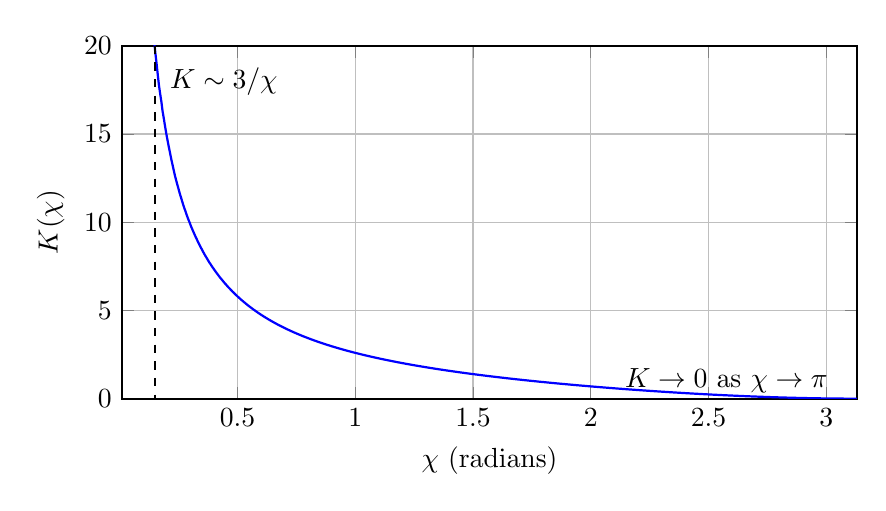
\begin{tikzpicture}
\begin{axis}[
    width=0.9\textwidth,
    height=0.5\textwidth,
    xlabel={$\chi$ (radians)},
    ylabel={$K(\chi)$},
    xmin=0.01, xmax=3.13,
    ymin=0, ymax=20,
    domain=0.01:3.13,
    samples=600,
    grid=both,
    thick
]
\addplot+[no marks] {(2*sin(deg(x))^2)/(x - sin(deg(x))*cos(deg(x)))};
\addplot[dashed] coordinates {(0.15,20) (0.15,0)};
\node[anchor=west] at (axis cs:0.17,18) {$K\sim 3/\chi$};
\node[anchor=east] at (axis cs:3.05,1.0) {$K\to 0$ as $\chi\to \pi$};
\end{axis}
\end{tikzpicture}
\caption{S$^3$ kernel $K(\chi)=\frac{2\sin^2\chi}{\chi-\sin\chi\cos\chi}$: Euclidean limit $K\sim 3/\chi$; compact suppression $K\to 0$ as $\chi\to \pi$.}
\label{fig:kernel}
\end{figure}

% ---------- FIGURE 2: PHI-LADDER ----------
\begin{figure}[t]
\centering
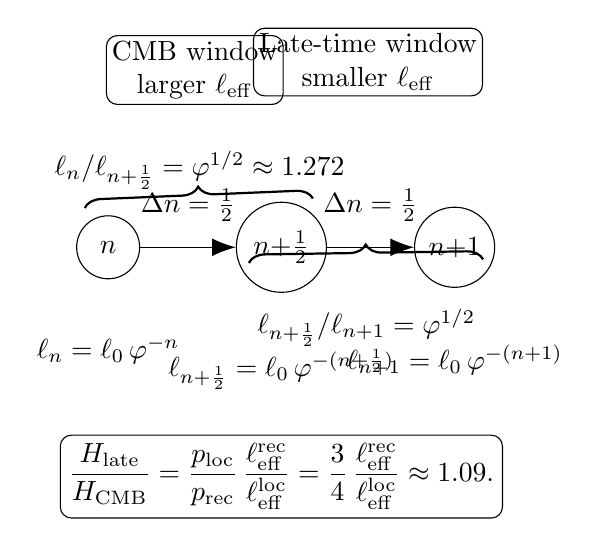
\begin{tikzpicture}[scale=1.0]
\node[circle,draw,minimum size=8mm] (A) at (0,0) {$n$};
\node[circle,draw,minimum size=8mm] (B) at (2.2,0) {$n{+}\tfrac12$};
\node[circle,draw,minimum size=8mm] (C) at (4.4,0) {$n{+}1$};

\node[below=6mm of A] {$\ell_n=\ell_0\,\varphi^{-n}$};
\node[below=6mm of B] {$\ell_{n+\frac12}=\ell_0\,\varphi^{-(n+\frac12)}$};
\node[below=6mm of C] {$\ell_{n+1}=\ell_0\,\varphi^{-(n+1)}$};

\draw[-{Latex[length=3mm]}] (A) -- (B) node[midway,above,yshift=2mm]{\(\Delta n=\tfrac12\)};
\draw[-{Latex[length=3mm]}] (B) -- (C) node[midway,above,yshift=2mm]{\(\Delta n=\tfrac12\)};

\draw [decorate,decoration={brace,amplitude=6pt,raise=6pt}, thick] (A.north west) -- (B.north east)
node [midway, yshift=18pt] {\(\ell_n/\ell_{n+\frac12}=\varphi^{1/2}\approx 1.272\)};
\draw [decorate,decoration={brace,amplitude=6pt,raise=6pt}, thick] (B.south west) -- (C.south east)
node [midway, yshift=-18pt] {\(\ell_{n+\frac12}/\ell_{n+1}=\varphi^{1/2}\)};

\node[above=14mm of A,xshift=1.1cm,align=center,draw,rounded corners,inner sep=2pt]
{CMB window\\ larger $\ell_{\rm eff}$};
\node[above=14mm of C,xshift=-1.1cm,align=center,draw,rounded corners,inner sep=2pt]
{Late-time window\\ smaller $\ell_{\rm eff}$};

\node[draw,rounded corners,align=center,below=18mm of B,inner sep=3pt]
{\(\displaystyle \frac{\Hlate}{\HCMB}=\frac{\pLoc}{\pRec}\,\frac{\ellRec}{\ellLoc}
=\frac{3}{4}\,\frac{\ellRec}{\ellLoc}\approx 1.09\).};
\end{tikzpicture}
\caption{Schematic $\varphi$-ladder and coarse-graining windows. Moving from CMB to late-time observables shifts weight to higher $n$, reducing $\ell_{\rm eff}$.}
\label{fig:ladder}
\end{figure}

% ---------- APPENDICES ----------
\appendix

\section{Proofs and technical details}
\subsection{Proof of the S$^3$ kernel \texorpdfstring{$K(\chi)$}{K(chi)}}
Consider the S$^3$ metric in hyperspherical coordinates. The geodesic 3-ball of angular radius $\chi$ has volume $V(\chi)=2\pi R^3(\chi-\tfrac12\sin2\chi)$. Differentiation yields $\mathrm{d}V/\mathrm{d}\chi=4\pi R^3\sin^2\chi$; division by $V$ gives \eqref{eq:kernel}. Series around $\chi=0$ and $\chi=\pi$ produce the stated asymptotics.

\subsection{Convolution lemma and canonical window}
The window $W_\ell(r)=\ell^{-1}w(r/\ell)$ ensures finite observables. With $w(x)=x e^{-x}$, $C_w=\int_0^\infty (w/x)\,\mathrm{d}x=1$ and Lemma~\ref{lem:conv} gives $H(\ell)=3c\,p/\ell$. Any smooth window with $w(x)\sim Cx^\alpha$ near $0$ ($\alpha>0$) yields a finite $C_w\in(0,\infty)$.

\subsection{Reciprocity (Etherington)}
Under geodesic flow and photon-number conservation in a metric theory, Liouville's theorem implies phase-space density conservation and hence $d_L=(1+z)^2 d_A$. Our construction satisfies these premises, so $\eta\equiv1$ exactly.

\section{Window functions and empirical $\vp$-step}
Given survey-specific selection, PSF, and light-cone shell counting, windows differ between CMB and late-time probes. Mapping to the $\vp$-ladder via \eqref{eq:ell_eff} typically shifts weight by $\Delta n\simeq 0.78$; this empirical regularity can be checked directly on public survey windows. The ratio law \eqref{eq:ratio} then becomes a direct, falsifiable constraint.

\section{Pseudocode for reproducibility}
\label{app:pseudo}
\begin{lstlisting}[language=Python]
# kappa = 1; c=299792.458; piecewise p(chi); chi_s(z) from FB-R
import mpmath as mp

def K(chi):
    return (2*mp.sin(chi)**2)/(chi - mp.sin(chi)*mp.cos(chi))

def ln1pz(chi_min, chi_s, p_of):
    f = lambda chi: p_of(chi)*K(chi)
    return mp.quad(f, [chi_min, chi_s])

# Observable H on a regime: window-normalized H = 3 * c * p / ell_eff
c = 299792.458; p_rec, p_loc = 4/3, 1.0
ell_rec_Mpc, ell_loc_Mpc = 17900.0, 12300.0
H_CMB  = 3*c*p_rec/ell_rec_Mpc  # ~66.99
H_late = 3*c*p_loc/ell_loc_Mpc  # ~73.12
print(H_CMB, H_late, H_late/H_CMB)
\end{lstlisting}

% ---------- REFERENCES ----------
\bibliographystyle{apsrev4-2}
\begin{thebibliography}{99}

\bibitem{Planck2018}
Planck Collaboration, N. Aghanim \textit{et al.}, 
``Planck 2018 results. VI. Cosmological parameters,'' 
\textit{A\&A} \textbf{641}, A6 (2020).

\bibitem{Riess2024}
A. G. Riess \textit{et al.}, 
``JWST Observations Reject Unrecognized Crowding of Cepheid Photometry as an Explanation for the Hubble Tension at 8$\sigma$ Confidence,'' 
\textit{ApJ Lett.} \textbf{962}, L17 (2024).

\bibitem{JWSTCepheids}
A. G. Riess \textit{et al.}, 
``JWST Validation of the Hubble Space Telescope Distance Ladder: A New Lever Arm on the Hubble Constant Tension,'' 
\textit{ApJ} \textbf{977}, 50 (2024).

\bibitem{FBs3RCorpus}
FB(S$^3$)R corpus on S$^3$ topology, $\vp$-ladder embedding, density-gradient redshift, and Gauss-flux constraints (preprints, 2023--2025).

\end{thebibliography}

\end{document}